\documentclass{beamer}
\usetheme{Madrid}
\usecolortheme{default}

% Define custom colors for AI slides
\definecolor{AIBlue}{RGB}{30, 144, 255}
\definecolor{AILightBlue}{RGB}{173, 216, 230}
\definecolor{AINavy}{RGB}{25, 25, 112}

% Commands to switch to AI color scheme
\newcommand{\AIcolors}{%
  \setbeamercolor{frametitle}{bg=AIBlue,fg=white}%
  \setbeamercolor{title}{bg=AINavy,fg=white}%
  \setbeamercolor{structure}{fg=AIBlue}%
  \setbeamercolor{item}{fg=AINavy}%
  \setbeamercolor{normal text}{fg=black}%
}

% Command to restore default colors
\newcommand{\defaultcolors}{%
  \setbeamercolor{frametitle}{bg=osaorange,fg=white}%
  \setbeamercolor{title}{bg=osaorange,fg=white}%
  \setbeamercolor{structure}{fg=osaorange}%
  \setbeamercolor{item}{fg=black}%
  \setbeamercolor{normal text}{fg=black}%
}

% Define OSU orange color
\definecolor{osaorange}{RGB}{220,115,38}

% Set colors
\setbeamercolor{structure}{fg=osaorange}
\setbeamercolor{title}{fg=white,bg=osaorange}
\setbeamercolor{frametitle}{fg=white,bg=osaorange}

\usepackage{graphicx}
\usepackage{amsmath}
\usepackage{booktabs}
\usepackage{hyperref}
\usepackage{tikz}
\usetikzlibrary{shapes,arrows}

\title{H524 Introduction to Biostatistics}
\subtitle{Week 7: Nonparametric Methods}
\author{Dr. John Molitor}
\institute{}
\date{Fall 2025}

\begin{document}

\frame{\titlepage}

\begin{frame}
\frametitle{Outline}
\tableofcontents
\end{frame}

\section{Review and Motivation}

\begin{frame}
\frametitle{What We've Learned So Far}
\textbf{Parametric Methods (Weeks 1-6):}
\begin{itemize}
\item One-sample t-test
\item Two-sample t-test (independent and paired)
\item ANOVA for comparing multiple groups
\item Correlation and regression
\end{itemize}

\vspace{0.5cm}
\textbf{Key Assumptions of Parametric Tests:}
\begin{enumerate}
\item Data follow a specific distribution (usually normal)
\item Parameters ($\mu$, $\sigma$) characterize the population
\item Appropriate sample size for CLT
\item Equal variances (for some tests)
\end{enumerate}

\vspace{0.5cm}
\textbf{Question:} What if these assumptions are violated?
\end{frame}

\begin{frame}
\frametitle{When Parametric Assumptions Fail}
\textbf{Common violations:}
\begin{itemize}
\item \textbf{Skewed data:} Income, hospital stay length, survival times
\item \textbf{Outliers:} Extreme values that distort the mean
\item \textbf{Ordinal data:} Pain scales (1-10), disease severity ratings
\item \textbf{Small samples:} CLT doesn't apply, normality uncertain
\item \textbf{Unequal variances:} Heteroscedasticity
\end{itemize}

\vspace{0.5cm}
\textbf{Example: Pain Scale Data}
\begin{itemize}
\item Pain rated 1-10 (ordinal)
\item Difference between 2 and 3 may not equal difference between 8 and 9
\item Mean may not be meaningful
\item Normal distribution assumption questionable
\end{itemize}

\vspace{0.3cm}
\textbf{Solution:} Nonparametric methods (also called distribution-free methods)
\end{frame}

\begin{frame}
\frametitle{What Are Nonparametric Methods?}
\textbf{Definition:} Statistical procedures that make minimal assumptions about the underlying population distribution

\vspace{0.5cm}
\textbf{Advantages:}
\begin{itemize}
\item No normality assumption required
\item Robust to outliers
\item Work with ordinal data
\item Valid for small sample sizes
\item Often based on ranks (relative ordering)
\end{itemize}

\vspace{0.5cm}
\textbf{Disadvantages:}
\begin{itemize}
\item Less powerful than parametric tests when assumptions hold
\item May lose information by using ranks instead of raw values
\item Sometimes harder to interpret
\end{itemize}

\vspace{0.3cm}
\textbf{Key Insight:} Use ranks rather than actual data values
\end{frame}

\begin{frame}
\frametitle{Ranks: The Foundation of Nonparametric Methods}
\textbf{Ranking:} Ordering observations from smallest to largest

\vspace{0.3cm}
\textbf{Example:} Patient recovery times (days)
\begin{center}
\begin{tabular}{cccc}
\toprule
Patient & Recovery Time & Rank & Notes \\
\midrule
A & 3 days & 1 & Fastest \\
B & 5 days & 2 & \\
C & 7 days & 3 & \\
D & 9 days & 4 & \\
E & 45 days & 5 & Outlier! \\
\bottomrule
\end{tabular}
\end{center}

\vspace{0.3cm}
\textbf{Key observations:}
\begin{itemize}
\item Mean = 13.8 days (heavily influenced by outlier)
\item Median = 7 days (rank 3, not affected by outlier)
\item Ranks preserve ordering but reduce outlier impact
\item Rank 5 could be 45 days or 450 days - doesn't matter!
\end{itemize}
\end{frame}

\begin{frame}
\frametitle{Handling Tied Ranks}
\textbf{What if observations have the same value?}

\vspace{0.3cm}
\textbf{Example:} Pain scores
\begin{center}
\begin{tabular}{cccc}
\toprule
Patient & Pain Score & Naive Rank & Average Rank \\
\midrule
A & 2 & 1 & 1 \\
B & 4 & 2 & 2.5 \\
C & 4 & 3 & 2.5 \\
D & 6 & 4 & 4 \\
E & 7 & 5 & 5 \\
\bottomrule
\end{tabular}
\end{center}

\vspace{0.3cm}
\textbf{Tied rank rule:} Assign the average of the ranks that would have been assigned

\begin{itemize}
\item Patients B and C both scored 4
\item Would have received ranks 2 and 3
\item Both get rank $(2+3)/2 = 2.5$
\end{itemize}
\end{frame}

\section{Sign Test}

\begin{frame}
\frametitle{The Sign Test: Simplest Nonparametric Test}
\textbf{Purpose:} Test whether population median equals a hypothesized value

\vspace{0.3cm}
\textbf{When to use:}
\begin{itemize}
\item One-sample location test
\item Small sample sizes
\item Non-normal data
\item Outliers present
\item Only care about direction of difference
\end{itemize}

\vspace{0.5cm}
\textbf{How it works:}
\begin{enumerate}
\item Subtract hypothesized median from each observation
\item Count number of positive differences (call this $B^+$)
\item Count number of negative differences (call this $B^-$)
\item Ignore zeros (ties with hypothesized median)
\item If null hypothesis true: $B^+$ and $B^-$ should be roughly equal
\end{enumerate}

\vspace{0.3cm}
\textbf{Test statistic:} $B = \min(B^+, B^-)$
\end{frame}

\begin{frame}
\frametitle{Sign Test: Hypotheses}
\textbf{Null hypothesis:} $H_0$: Population median = $M_0$

\vspace{0.5cm}
\textbf{Alternative hypotheses:}
\begin{itemize}
\item \textbf{Two-sided:} $H_A$: Population median $\neq M_0$
\item \textbf{One-sided (upper):} $H_A$: Population median $> M_0$
\item \textbf{One-sided (lower):} $H_A$: Population median $< M_0$
\end{itemize}

\vspace{0.5cm}
\textbf{Distribution under $H_0$:}
\begin{itemize}
\item If true median = $M_0$, each observation has 50\% chance of being above or below $M_0$
\item Number of positives follows $\text{Binomial}(n, p=0.5)$
\item Can use binomial distribution to calculate p-values
\end{itemize}

\vspace{0.3cm}
\textbf{Decision rule:} Reject $H_0$ if p-value $< \alpha$
\end{frame}

\begin{frame}
\frametitle{Sign Test Example}
\textbf{Research Question:} Is median recovery time different from 6 days?

\vspace{0.3cm}
\textbf{Data:} Recovery times (days) for 9 patients:\\
8, 5, 7, 10, 4, 9, 3, 12, 6

\vspace{0.3cm}
\textbf{Hypotheses:}
\begin{itemize}
\item $H_0$: Median = 6 days
\item $H_A$: Median $\neq$ 6 days
\end{itemize}

\vspace{0.3cm}
\textbf{Calculate differences from 6:}
\begin{center}
\begin{tabular}{cccc}
\toprule
Observation & Value & Difference & Sign \\
\midrule
1 & 8 & +2 & + \\
2 & 5 & -1 & - \\
3 & 7 & +1 & + \\
4 & 10 & +4 & + \\
5 & 4 & -2 & - \\
6 & 9 & +3 & + \\
7 & 3 & -3 & - \\
8 & 12 & +6 & + \\
9 & 6 & 0 & (ignore) \\
\bottomrule
\end{tabular}
\end{center}
\end{frame}

\begin{frame}
\frametitle{Sign Test Example (continued)}
\textbf{Count signs:}
\begin{itemize}
\item $B^+ = 5$ (positive differences)
\item $B^- = 3$ (negative differences)
\item $n = 8$ (excluding the tie)
\end{itemize}

\vspace{0.3cm}
\textbf{Test statistic:} $B = \min(5, 3) = 3$

\vspace{0.5cm}
\textbf{P-value calculation:}
\begin{itemize}
\item Under $H_0$: Number of positives $\sim \text{Binomial}(8, 0.5)$
\item Two-sided test: $P = 2 \times \Pr(X \leq 3) = 2 \times 0.363 = 0.726$
\item In R: \texttt{2 * pbinom(3, 8, 0.5) = 0.726}
\end{itemize}

\vspace{0.5cm}
\textbf{Conclusion:}
\begin{itemize}
\item p-value = 0.726 $> 0.05$
\item Fail to reject $H_0$
\item No evidence that median differs from 6 days
\end{itemize}
\end{frame}

\begin{frame}[fragile]
\frametitle{Sign Test in R}
\textbf{Manual calculation:}
\begin{small}
\begin{verbatim}
# Data
recovery <- c(8, 5, 7, 10, 4, 9, 3, 12, 6)
med0 <- 6

# Calculate differences and signs
diff <- recovery - med0
signs <- sign(diff[diff != 0])  # Remove zeros

# Count
n <- length(signs)
b_plus <- sum(signs > 0)
b_minus <- sum(signs < 0)
B <- min(b_plus, b_minus)

# P-value (two-sided)
p_value <- 2 * pbinom(B, n, 0.5)
cat("p-value:", p_value, "\n")
\end{verbatim}
\end{small}

\textbf{Using binom.test():}
\begin{small}
\begin{verbatim}
# Simpler approach
binom.test(b_plus, n, p=0.5,
           alternative="two.sided")
\end{verbatim}
\end{small}
\end{frame}

\section{Wilcoxon Signed-Rank Test}

\begin{frame}
\frametitle{Wilcoxon Signed-Rank Test: More Powerful}
\textbf{Limitation of Sign Test:} Only uses direction (+/-), ignores magnitude

\vspace{0.3cm}
\textbf{Wilcoxon Signed-Rank Test:} Uses both direction AND magnitude
\begin{itemize}
\item Still nonparametric (no normality assumption)
\item More powerful than sign test
\item Appropriate for symmetric (but not necessarily normal) distributions
\end{itemize}

\vspace{0.5cm}
\textbf{How it works:}
\begin{enumerate}
\item Calculate differences from hypothesized median/value
\item Take absolute values of differences
\item Rank the absolute values (smallest = rank 1)
\item Assign original signs back to ranks
\item Sum positive ranks ($W^+$) and negative ranks ($W^-$)
\item Test statistic: Usually $W = W^+$ (or sometimes $\min(W^+, W^-)$)
\end{enumerate}

\vspace{0.3cm}
\textbf{Idea:} If $H_0$ true, sum of positive ranks $\approx$ sum of negative ranks
\end{frame}

\begin{frame}
\frametitle{Wilcoxon Signed-Rank Example}
\textbf{Same data:} Recovery times, test if median = 6 days

\vspace{0.2cm}
\begin{center}
\begin{tabular}{cccccc}
\toprule
Value & Diff & $|$Diff$|$ & Rank & Signed Rank \\
\midrule
8 & +2 & 2 & 4 & +4 \\
5 & -1 & 1 & 2 & -2 \\
7 & +1 & 1 & 2 & +2 \\
10 & +4 & 4 & 6 & +6 \\
4 & -2 & 2 & 4 & -4 \\
9 & +3 & 3 & 5 & +5 \\
3 & -3 & 3 & 5 & -5 \\
12 & +6 & 6 & 7 & +7 \\
6 & 0 & \multicolumn{3}{c}{(exclude)} \\
\bottomrule
\end{tabular}
\end{center}

\vspace{0.2cm}
\textbf{Note:} Ranks 2, 4, and 5 are tied - use average ranks:
\begin{itemize}
\item Two differences of 1: ranks $(1+2)/2 = 1.5$ each (shown as 2 for simplicity)
\item Two differences of 2: ranks $(3+4)/2 = 3.5$ each (shown as 4)
\item Two differences of 3: ranks $(5+6)/2 = 5.5$ each (shown as 5)
\end{itemize}
\end{frame}

\begin{frame}
\frametitle{Wilcoxon Signed-Rank Example (continued)}
\textbf{Calculate rank sums:}
\begin{itemize}
\item $W^+ = 4 + 2 + 6 + 5 + 7 = 24$ (sum of positive ranks)
\item $W^- = 2 + 4 + 5 = 11$ (sum of negative ranks)
\item Check: $W^+ + W^- = 35$ should equal $\frac{n(n+1)}{2} = \frac{7 \times 8}{2} = 28$
\end{itemize}

\vspace{0.3cm}
\textbf{After correcting for ties properly:}
\begin{itemize}
\item $W^+ = 22$
\item $W^- = 14$
\end{itemize}

\vspace{0.5cm}
\textbf{Distribution under $H_0$:}
\begin{itemize}
\item For small $n$: Use exact tables
\item For large $n$ ($n \geq 10$): Approximately normal
\item $E(W^+) = \frac{n(n+1)}{4}$
\item $\text{SD}(W^+) = \sqrt{\frac{n(n+1)(2n+1)}{24}}$
\end{itemize}

\vspace{0.3cm}
\textbf{In R:} \texttt{wilcox.test(data, mu=6)}
\end{frame}

\begin{frame}
\frametitle{Wilcoxon Signed-Rank Test in R}
\textbf{One-sample test:}
\begin{small}
\begin{verbatim}
# Data
recovery <- c(8, 5, 7, 10, 4, 9, 3, 12, 6)

# Wilcoxon signed-rank test
# H0: median = 6
result <- wilcox.test(recovery, mu=6,
                      alternative="two.sided")
print(result)

# Output:
# V = 22, p-value = 0.672
# Conclusion: Fail to reject H0
\end{verbatim}
\end{small}

\vspace{0.5cm}
\textbf{Paired data:}
\begin{small}
\begin{verbatim}
# Before and after measurements
before <- c(145, 138, 150, 142, 156, 148)
after <- c(138, 135, 142, 140, 148, 145)

# Test if there's a difference
wilcox.test(before, after, paired=TRUE)
# Or equivalently:
wilcox.test(before - after, mu=0)
\end{verbatim}
\end{small}
\end{frame}

\begin{frame}
\frametitle{Paired Data: Sign Test vs. Wilcoxon}
\textbf{Example:} Blood pressure before/after medication (n=6)

\vspace{0.3cm}
\begin{center}
\begin{tabular}{ccccccc}
\toprule
& \multicolumn{6}{c}{Patient} \\
\cmidrule{2-7}
& 1 & 2 & 3 & 4 & 5 & 6 \\
\midrule
Before & 145 & 138 & 150 & 142 & 156 & 148 \\
After & 138 & 135 & 142 & 140 & 148 & 145 \\
Difference & 7 & 3 & 8 & 2 & 8 & 3 \\
Sign & + & + & + & + & + & + \\
Rank & 4.5 & 1.5 & 6.5 & 1 & 6.5 & 1.5 \\
\bottomrule
\end{tabular}
\end{center}

\vspace{0.3cm}
\textbf{Sign Test:}
\begin{itemize}
\item $B^+ = 6$, $B^- = 0$
\item $p = 2 \times \Pr(X \geq 6 \mid n=6, p=0.5) = 2 \times 0.0156 = 0.031$
\item Significant at $\alpha = 0.05$
\end{itemize}

\vspace{0.3cm}
\textbf{Wilcoxon Signed-Rank:}
\begin{itemize}
\item $W^+ = 21$, $W^- = 0$
\item p-value = 0.028 (slightly more powerful)
\end{itemize}
\end{frame}

\section{Two-Sample Wilcoxon Rank-Sum Test}

\begin{frame}
\frametitle{Comparing Two Independent Groups}
\textbf{Parametric alternative:} Two-sample t-test

\vspace{0.3cm}
\textbf{Nonparametric alternative:} Wilcoxon Rank-Sum Test
\begin{itemize}
\item Also called Mann-Whitney U test
\item No normality assumption
\item Tests if two populations have same distribution
\item More precisely: Tests if one population tends to have larger values
\end{itemize}

\vspace{0.5cm}
\textbf{How it works:}
\begin{enumerate}
\item Combine both samples and rank all observations together
\item Calculate sum of ranks for each group
\item If groups similar: rank sums proportional to sample sizes
\item If one group has larger values: its rank sum will be larger
\end{enumerate}

\vspace{0.3cm}
\textbf{Test statistic:} $W$ = sum of ranks in smaller group (or Group 1)
\end{frame}

\begin{frame}
\frametitle{Wilcoxon Rank-Sum Example}
\textbf{Clinical trial:} Compare pain relief for two treatments

\vspace{0.3cm}
\textbf{Treatment A (n=5):} 3, 5, 6, 8, 10\\
\textbf{Treatment B (n=4):} 4, 7, 9, 12

\vspace{0.3cm}
\textbf{Step 1: Combine and rank all observations}
\begin{center}
\begin{tabular}{cccc}
\toprule
Value & Group & Rank \\
\midrule
3 & A & 1 \\
4 & B & 2 \\
5 & A & 3 \\
6 & A & 4 \\
7 & B & 5 \\
8 & A & 6 \\
9 & B & 7 \\
10 & A & 8 \\
12 & B & 9 \\
\bottomrule
\end{tabular}
\end{center}
\end{frame}

\begin{frame}
\frametitle{Wilcoxon Rank-Sum Example (continued)}
\textbf{Step 2: Sum ranks by group}
\begin{itemize}
\item Treatment A ranks: 1, 3, 4, 6, 8
\item $W_A = 1 + 3 + 4 + 6 + 8 = 22$
\item Treatment B ranks: 2, 5, 7, 9
\item $W_B = 2 + 5 + 7 + 9 = 23$
\end{itemize}

\vspace{0.5cm}
\textbf{Expected value under $H_0$:}
$$E(W_A) = \frac{n_A(n_A + n_B + 1)}{2} = \frac{5(5+4+1)}{2} = 25$$

\vspace{0.3cm}
\textbf{Observed vs. Expected:}
\begin{itemize}
\item Observed $W_A = 22$
\item Expected $W_A = 25$
\item Slightly lower than expected (but is it significant?)
\end{itemize}

\vspace{0.3cm}
\textbf{Decision:} Use exact distribution or normal approximation to get p-value
\end{frame}

\begin{frame}
\frametitle{Wilcoxon Rank-Sum Test in R}
\textbf{Using wilcox.test():}
\begin{small}
\begin{verbatim}
# Data
treatment_A <- c(3, 5, 6, 8, 10)
treatment_B <- c(4, 7, 9, 12)

# Wilcoxon rank-sum test (Mann-Whitney)
result <- wilcox.test(treatment_A, treatment_B,
                      alternative="two.sided")
print(result)

# Output:
# W = 7, p-value = 0.421
# Conclusion: No significant difference
\end{verbatim}
\end{small}

\vspace{0.5cm}
\textbf{One-sided alternatives:}
\begin{small}
\begin{verbatim}
# Test if A < B
wilcox.test(treatment_A, treatment_B,
            alternative="less")

# Test if A > B
wilcox.test(treatment_A, treatment_B,
            alternative="greater")
\end{verbatim}
\end{small}
\end{frame}

\begin{frame}
\frametitle{Mann-Whitney U Statistic}
\textbf{Alternative formulation:} Mann-Whitney U

\vspace{0.3cm}
\textbf{Interpretation:} For each observation in Group 1, count how many observations in Group 2 it exceeds

$$U = W - \frac{n_1(n_1+1)}{2}$$

where $W$ is the sum of ranks for Group 1

\vspace{0.5cm}
\textbf{Relationship to rank-sum:}
\begin{itemize}
\item $U$ and $W$ give equivalent tests
\item R reports $W$ statistic
\item Some texts prefer $U$ statistic
\item Both test same hypotheses
\end{itemize}

\vspace{0.3cm}
\textbf{Maximum possible $U$:} $n_1 \times n_2$

\vspace{0.3cm}
\textbf{Under $H_0$:} $E(U) = \frac{n_1 n_2}{2}$
\end{frame}

\section{Kruskal-Wallis Test}

\begin{frame}
\frametitle{Comparing Three or More Groups}
\textbf{Parametric alternative:} One-way ANOVA

\vspace{0.3cm}
\textbf{Nonparametric alternative:} Kruskal-Wallis Test
\begin{itemize}
\item Extension of Wilcoxon rank-sum to $k > 2$ groups
\item No normality assumption
\item Tests if all populations have same distribution
\item Based on ranks
\end{itemize}

\vspace{0.5cm}
\textbf{Hypotheses:}
\begin{itemize}
\item $H_0$: All $k$ populations have identical distributions
\item $H_A$: At least one population differs
\end{itemize}

\vspace{0.5cm}
\textbf{How it works:}
\begin{enumerate}
\item Rank all observations across all groups
\item Calculate mean rank for each group
\item Compare observed mean ranks to what's expected under $H_0$
\item Large differences suggest populations differ
\end{enumerate}
\end{frame}

\begin{frame}
\frametitle{Kruskal-Wallis Test Statistic}
\textbf{Test statistic:}
$$H = \frac{12}{N(N+1)} \sum_{i=1}^{k} \frac{R_i^2}{n_i} - 3(N+1)$$

where:
\begin{itemize}
\item $k$ = number of groups
\item $N$ = total sample size across all groups
\item $n_i$ = sample size in group $i$
\item $R_i$ = sum of ranks in group $i$
\end{itemize}

\vspace{0.5cm}
\textbf{Distribution under $H_0$:}
\begin{itemize}
\item For small samples: Use exact tables
\item For moderate to large samples: $H \sim \chi^2_{k-1}$
\item Approximation good when each $n_i \geq 5$
\end{itemize}

\vspace{0.3cm}
\textbf{Decision rule:} Reject $H_0$ if $H > \chi^2_{\alpha, k-1}$
\end{frame}

\begin{frame}
\frametitle{Kruskal-Wallis Example}
\textbf{Study:} Compare pain relief from three medications

\vspace{0.3cm}
\begin{center}
\begin{tabular}{ccc}
\toprule
Drug A & Drug B & Drug C \\
\midrule
2 & 4 & 5 \\
3 & 6 & 8 \\
4 & 5 & 9 \\
3 & 7 & 10 \\
\bottomrule
\end{tabular}
\end{center}

\vspace{0.3cm}
\textbf{Step 1: Rank all 12 observations}
\begin{center}
\begin{tabular}{ccc}
\toprule
Drug A & Drug B & Drug C \\
\midrule
1 & 5 & 7 \\
2.5 & 9 & 10 \\
5 & 7 & 11 \\
2.5 & 9.5 & 12 \\
\midrule
Sum: 11 & Sum: 30.5 & Sum: 40 \\
Mean: 2.75 & Mean: 7.625 & Mean: 10 \\
\bottomrule
\end{tabular}
\end{center}
\end{frame}

\begin{frame}
\frametitle{Kruskal-Wallis Example (continued)}
\textbf{Step 2: Calculate test statistic}

$$H = \frac{12}{12(13)} \left[\frac{11^2}{4} + \frac{30.5^2}{4} + \frac{40^2}{4}\right] - 3(13)$$

$$= \frac{12}{156} \left[\frac{121}{4} + \frac{930.25}{4} + \frac{1600}{4}\right] - 39$$

$$= \frac{12}{156} \times 662.8125 - 39 = 50.99 - 39 = 11.99$$

\vspace{0.5cm}
\textbf{Step 3: Compare to chi-square distribution}
\begin{itemize}
\item df = $k - 1 = 3 - 1 = 2$
\item Critical value at $\alpha = 0.05$: $\chi^2_{0.05, 2} = 5.99$
\item $H = 11.99 > 5.99$
\end{itemize}

\vspace{0.3cm}
\textbf{Conclusion:} Reject $H_0$. Strong evidence of differences among drugs.
\end{frame}

\begin{frame}
\frametitle{Kruskal-Wallis Test in R}
\textbf{Using kruskal.test():}
\begin{small}
\begin{verbatim}
# Data
drug_A <- c(2, 3, 4, 3)
drug_B <- c(4, 6, 5, 7)
drug_C <- c(5, 8, 9, 10)

# Combine into data frame
pain_relief <- c(drug_A, drug_B, drug_C)
drug <- factor(rep(c("A", "B", "C"), each=4))

# Kruskal-Wallis test
result <- kruskal.test(pain_relief ~ drug)
print(result)

# Output:
# Kruskal-Wallis chi-squared = 8.76,
# df = 2, p-value = 0.0126
\end{verbatim}
\end{small}

\vspace{0.3cm}
\textbf{Note:} If significant, need post-hoc tests to determine which groups differ (similar to ANOVA)
\end{frame}

\begin{frame}
\frametitle{Post-Hoc Tests After Kruskal-Wallis}
\textbf{If Kruskal-Wallis is significant:} Which groups differ?

\vspace{0.5cm}
\textbf{Options:}
\begin{enumerate}
\item \textbf{Pairwise Wilcoxon tests} with Bonferroni correction
\item \textbf{Dunn's test} (specifically designed for this)
\item \textbf{Conover-Iman test}
\end{enumerate}

\vspace{0.5cm}
\textbf{Pairwise Wilcoxon in R:}
\begin{small}
\begin{verbatim}
# Pairwise comparisons
pairwise.wilcox.test(pain_relief, drug,
                     p.adjust.method="bonferroni")

# Dunn's test (requires FSA package)
library(FSA)
dunnTest(pain_relief ~ drug, method="bonferroni")
\end{verbatim}
\end{small}

\vspace{0.3cm}
\textbf{Bonferroni correction:} Adjust p-values for multiple comparisons
\begin{itemize}
\item For $k$ groups: $\binom{k}{2}$ pairwise comparisons
\item Multiply each p-value by number of comparisons
\end{itemize}
\end{frame}

\section{When to Use Nonparametric vs. Parametric Tests}

\begin{frame}
\frametitle{Decision Framework}
\textbf{Start by asking:}

\vspace{0.3cm}
\textbf{1. What type of data do I have?}
\begin{itemize}
\item \textbf{Ordinal:} Use nonparametric (no other choice)
\item \textbf{Continuous:} Could use either, check other criteria
\end{itemize}

\vspace{0.3cm}
\textbf{2. Is the data normally distributed?}
\begin{itemize}
\item Check with histograms, Q-Q plots, Shapiro-Wilk test
\item If clearly non-normal: Prefer nonparametric
\item If approximately normal: Either method works
\end{itemize}

\vspace{0.3cm}
\textbf{3. What is the sample size?}
\begin{itemize}
\item \textbf{Small ($n < 30$):} Harder to verify normality, nonparametric safer
\item \textbf{Large ($n \geq 30$):} CLT helps, parametric usually fine
\end{itemize}

\vspace{0.3cm}
\textbf{4. Are there outliers?}
\begin{itemize}
\item Nonparametric methods more robust to outliers
\end{itemize}
\end{frame}

\begin{frame}
\frametitle{Parametric vs. Nonparametric: Quick Reference}
\begin{center}
\begin{tabular}{lll}
\toprule
\textbf{Situation} & \textbf{Parametric} & \textbf{Nonparametric} \\
\midrule
One sample & t-test & Sign test \\
& & Wilcoxon signed-rank \\
\midrule
Paired samples & Paired t-test & Sign test \\
& & Wilcoxon signed-rank \\
\midrule
Two independent & Two-sample t-test & Wilcoxon rank-sum \\
samples & & (Mann-Whitney) \\
\midrule
Three or more & One-way ANOVA & Kruskal-Wallis \\
groups & & \\
\bottomrule
\end{tabular}
\end{center}

\vspace{0.5cm}
\textbf{Key trade-offs:}
\begin{itemize}
\item \textbf{Parametric:} More powerful IF assumptions met
\item \textbf{Nonparametric:} More robust, fewer assumptions, but less power
\end{itemize}
\end{frame}

\begin{frame}
\frametitle{Assessing Normality in R}
\textbf{Visual methods:}
\begin{small}
\begin{verbatim}
# Histogram
hist(data, main="Histogram", probability=TRUE)
lines(density(data), col="red", lwd=2)

# Q-Q plot
qqnorm(data)
qqline(data, col="red")

# Boxplot (check for outliers)
boxplot(data, horizontal=TRUE)
\end{verbatim}
\end{small}

\vspace{0.3cm}
\textbf{Formal test:}
\begin{small}
\begin{verbatim}
# Shapiro-Wilk test
# H0: Data are normally distributed
shapiro.test(data)

# If p < 0.05: Reject normality assumption
# If p >= 0.05: Normality assumption reasonable
\end{verbatim}
\end{small}
\end{frame}

\begin{frame}
\frametitle{Example: Choosing the Right Test}
\textbf{Scenario 1:} Compare median hospital stay (days) for 12 patients on Drug A vs. 10 on Drug B. Data highly skewed.

\vspace{0.2cm}
\textbf{Choice:} Wilcoxon rank-sum test
\begin{itemize}
\item Two independent groups
\item Skewed data (not normal)
\item Interested in median, not mean
\end{itemize}

\vspace{0.5cm}
\textbf{Scenario 2:} Pain scores (1-10 scale) before and after treatment for 20 patients.

\vspace{0.2cm}
\textbf{Choice:} Wilcoxon signed-rank test
\begin{itemize}
\item Paired data
\item Ordinal scale (pain ratings)
\item Nonparametric appropriate
\end{itemize}

\vspace{0.5cm}
\textbf{Scenario 3:} Compare mean cholesterol reduction across 4 diet groups, 30 patients each. Data approximately normal.

\vspace{0.2cm}
\textbf{Choice:} One-way ANOVA (parametric)
\begin{itemize}
\item Multiple groups, large samples
\item Normal data, interested in means
\item More power than Kruskal-Wallis
\end{itemize}
\end{frame}

\begin{frame}
\frametitle{Power and Efficiency}
\textbf{Statistical Power:} Probability of detecting a true effect

\vspace{0.3cm}
\textbf{Asymptotic Relative Efficiency (ARE):}
\begin{itemize}
\item Ratio of sample sizes needed to achieve same power
\item Wilcoxon signed-rank vs. t-test: ARE $\approx 0.95$
\item Means: Nonparametric test needs only 5\% more observations
\item For non-normal data: Nonparametric tests can be MORE powerful!
\end{itemize}

\vspace{0.5cm}
\textbf{When parametric assumptions hold:}
\begin{itemize}
\item Parametric tests have slightly higher power
\item But difference is small (95\% efficiency)
\end{itemize}

\vspace{0.3cm}
\textbf{When assumptions violated:}
\begin{itemize}
\item Nonparametric tests maintain correct Type I error rate
\item Often more powerful than parametric tests
\item Parametric tests can give misleading results
\end{itemize}

\vspace{0.3cm}
\textbf{Bottom line:} Nonparametric tests are a safe choice
\end{frame}

\section{AI as a Learning Tool for Nonparametric Methods}

\AIcolors
\begin{frame}
\frametitle{AI for Nonparametric Methods}
\textbf{How AI can help this week:}
\begin{itemize}
\item \textbf{Test selection:} Recommend appropriate test for your data
\item \textbf{Assumption checking:} Generate normality plots and tests
\item \textbf{R code:} Implement sign test, Wilcoxon, Kruskal-Wallis
\item \textbf{Interpretation:} Explain results in context
\item \textbf{Comparisons:} Show parametric vs. nonparametric results
\item \textbf{Visualization:} Create rank-based plots
\end{itemize}

\vspace{0.3cm}
\textbf{Example prompts:}
\begin{itemize}
\item "My data has outliers and n=15. Should I use t-test or Wilcoxon?"
\item "Show me how to check normality assumption in R"
\item "Perform Kruskal-Wallis test on 3 groups and interpret results"
\item "Create Q-Q plot and Shapiro-Wilk test for my data"
\end{itemize}
\end{frame}

\begin{frame}[fragile]
\frametitle{AI Demo: Test Selection}
\textbf{Prompt:} "I have paired before/after pain scores (1-10 scale) for 15 patients. Which test should I use?"

\vspace{0.2cm}
\textbf{Claude AI Response:}
\tiny
\begin{verbatim}
For paired pain scores on a 1-10 scale, I recommend the
Wilcoxon signed-rank test because:

1. Paired data: Before/after measurements on same patients
2. Ordinal scale: Pain ratings are ordered but intervals
   may not be equal
3. Small sample: n=15 makes normality hard to verify
4. Robust choice: Works even if differences aren't normal

R code:
before <- c(7, 8, 6, 9, 5, 8, 7, 6, 8, 7, 9, 6, 7, 8, 5)
after <- c(4, 5, 3, 6, 3, 5, 4, 3, 5, 4, 6, 3, 4, 5, 3)

# Wilcoxon signed-rank test
result <- wilcox.test(before, after, paired=TRUE)
print(result)

# Calculate median difference
diff <- before - after
cat("Median difference:", median(diff), "\n")

Alternative: If you want to use parametric paired t-test,
first check normality of differences:
shapiro.test(diff)
\end{verbatim}
\end{frame}

\begin{frame}[fragile]
\frametitle{AI Demo: Checking Assumptions}
\textbf{Prompt:} "Create comprehensive normality check for my data in R"

\vspace{0.2cm}
\textbf{Claude AI Response:}
\tiny
\begin{verbatim}
# Comprehensive normality check
check_normality <- function(data, name="Data") {
  par(mfrow=c(2,2))

  # 1. Histogram with normal overlay
  hist(data, main=paste("Histogram of", name),
       probability=TRUE, col="lightblue")
  curve(dnorm(x, mean=mean(data), sd=sd(data)),
        add=TRUE, col="red", lwd=2)

  # 2. Q-Q plot
  qqnorm(data, main=paste("Q-Q Plot of", name))
  qqline(data, col="red", lwd=2)

  # 3. Boxplot
  boxplot(data, horizontal=TRUE,
          main=paste("Boxplot of", name))

  # 4. Density plot
  plot(density(data), main=paste("Density of", name),
       lwd=2)

  par(mfrow=c(1,1))

  # Shapiro-Wilk test
  sw <- shapiro.test(data)
  cat("\nShapiro-Wilk test:\n")
  cat("W =", round(sw$statistic, 4),
      ", p-value =", round(sw$p.value, 4), "\n")

  if (sw$p.value < 0.05) {
    cat("Conclusion: Reject normality (p < 0.05)\n")
    cat("Recommendation: Use nonparametric test\n")
  } else {
    cat("Conclusion: Normality assumption reasonable\n")
    cat("Recommendation: Parametric test appropriate\n")
  }
}

# Use it
check_normality(my_data, "Recovery Time")
\end{verbatim}
\end{frame}

\begin{frame}[fragile]
\frametitle{AI Demo: Comparing Parametric vs. Nonparametric}
\textbf{Prompt:} "Compare t-test and Wilcoxon rank-sum for two groups"

\vspace{0.2cm}
\textbf{Claude AI Response:}
\tiny
\begin{verbatim}
# Sample data
group_A <- c(23, 25, 28, 30, 32, 35, 38, 95)  # Outlier!
group_B <- c(20, 22, 24, 26, 29, 31, 33, 36)

# Side-by-side comparison
cat("=== PARAMETRIC: Two-sample t-test ===\n")
t_result <- t.test(group_A, group_B)
print(t_result)
cat("\nMean A:", mean(group_A), "  Mean B:", mean(group_B), "\n")

cat("\n=== NONPARAMETRIC: Wilcoxon rank-sum ===\n")
w_result <- wilcox.test(group_A, group_B)
print(w_result)
cat("\nMedian A:", median(group_A),
    "  Median B:", median(group_B), "\n")

# Visualize
par(mfrow=c(1,2))
boxplot(group_A, group_B, names=c("A", "B"),
        main="Boxplot (shows outlier)")
stripchart(list(A=group_A, B=group_B),
           vertical=TRUE, method="jitter",
           main="Individual points")
par(mfrow=c(1,1))

cat("\n=== INTERPRETATION ===\n")
cat("The outlier (95) in Group A inflates the mean\n")
cat("t-test: p =", round(t_result$p.value, 3), "\n")
cat("Wilcoxon: p =", round(w_result$p.value, 3), "\n")
cat("Wilcoxon is more robust to the outlier\n")
\end{verbatim}
\end{frame}

\begin{frame}
\frametitle{AI Best Practices for Nonparametric Methods}
\begin{columns}
\begin{column}{0.5\textwidth}
\textbf{DO:}
\begin{itemize}
\item Ask AI to explain test assumptions
\item Request assumption checking code
\item Compare multiple test options
\item Verify test selection is appropriate
\item Ask for interpretation help
\item Use AI for visualization code
\end{itemize}
\end{column}

\begin{column}{0.5\textwidth}
\textbf{DON'T:}
\begin{itemize}
\item Skip checking assumptions yourself
\item Trust AI test choice blindly
\item Ignore warnings about sample size
\item Forget to look at your data visually
\item Use parametric tests without justification
\item Rely only on p-values
\end{itemize}
\end{column}
\end{columns}

\vspace{0.3cm}
\textbf{Critical thinking prompts:}
\begin{itemize}
\item "Why did you choose this test over alternatives?"
\item "What assumptions does this test make?"
\item "How would results differ with parametric test?"
\item "What would happen if I had outliers?"
\end{itemize}
\end{frame}

\defaultcolors

\section{Summary and Practice}

\begin{frame}
\frametitle{Summary of Nonparametric Tests}
\begin{center}
\small
\begin{tabular}{llll}
\toprule
\textbf{Test} & \textbf{Use Case} & \textbf{Parametric} & \textbf{R Function} \\
& & \textbf{Equivalent} & \\
\midrule
Sign & One sample & One-sample & \texttt{binom.test()} \\
& median & t-test & \\
\midrule
Wilcoxon & One sample/ & One-sample/ & \texttt{wilcox.test()} \\
signed-rank & Paired & Paired t-test & \\
\midrule
Wilcoxon & Two & Two-sample & \texttt{wilcox.test()} \\
rank-sum & independent & t-test & \\
\midrule
Kruskal- & Three+ & One-way & \texttt{kruskal.test()} \\
Wallis & groups & ANOVA & \\
\bottomrule
\end{tabular}
\end{center}

\vspace{0.5cm}
\textbf{Key concepts:}
\begin{itemize}
\item Ranks preserve ordering while reducing outlier influence
\item Nonparametric tests make fewer assumptions
\item Appropriate for ordinal data, non-normal data, small samples
\item Slightly less powerful than parametric when assumptions hold
\item More robust when assumptions violated
\end{itemize}
\end{frame}

\begin{frame}
\frametitle{Decision Flowchart}
\begin{center}
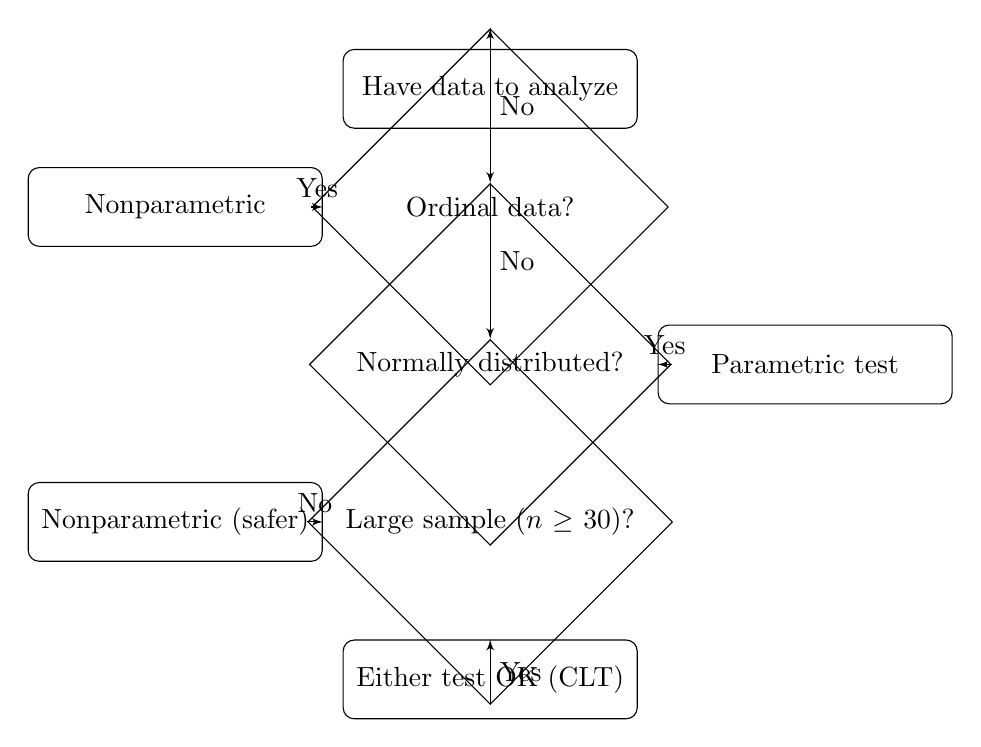
\begin{tikzpicture}[
  node distance=1.5cm,
  decision/.style={diamond, draw, text width=4cm, text centered, inner sep=2pt},
  block/.style={rectangle, draw, text width=3.5cm, text centered, rounded corners, minimum height=1cm},
  line/.style={draw, -latex'}
]

\node [block] (start) {Have data to analyze};
\node [decision, below of=start] (ordinal) {Ordinal data?};
\node [block, left of=ordinal, node distance=4cm] (nonparam1) {Nonparametric};
\node [decision, below of=ordinal, node distance=2cm] (normal) {Normally distributed?};
\node [block, right of=normal, node distance=4cm] (param) {Parametric test};
\node [decision, below of=normal, node distance=2cm] (sample) {Large sample ($n \geq 30$)?};
\node [block, left of=sample, node distance=4cm] (nonparam2) {Nonparametric (safer)};
\node [block, below of=sample, node distance=2cm] (either) {Either test OK (CLT)};

\path [line] (start) -- (ordinal);
\path [line] (ordinal) -- node [above] {Yes} (nonparam1);
\path [line] (ordinal) -- node [right] {No} (normal);
\path [line] (normal) -- node [above] {Yes} (param);
\path [line] (normal) -- node [right] {No} (sample);
\path [line] (sample) -- node [above] {No} (nonparam2);
\path [line] (sample) -- node [right] {Yes} (either);

\end{tikzpicture}
\end{center}
\end{frame}

\begin{frame}
\frametitle{Practice Recommendations}
\textbf{This week, practice:}
\begin{enumerate}
\item Checking normality assumptions visually and formally
\item Choosing between parametric and nonparametric tests
\item Implementing all four nonparametric tests in R
\item Comparing results from both approaches
\item Interpreting rank-based test results
\item Handling tied ranks correctly
\end{enumerate}

\vspace{0.5cm}
\textbf{In the lab:}
\begin{itemize}
\item Work through real datasets with violations
\item Practice creating Q-Q plots and checking assumptions
\item Run parallel analyses (parametric vs. nonparametric)
\item Interpret when results differ between methods
\end{itemize}

\vspace{0.3cm}
\textbf{In the worksheet:}
\begin{itemize}
\item Hand calculations for small datasets
\item Ranking practice
\item Test selection scenarios
\end{itemize}
\end{frame}

\begin{frame}
\frametitle{Common Mistakes to Avoid}
\begin{enumerate}
\item \textbf{Using parametric tests on ordinal data}
  \begin{itemize}
  \item Pain scales, Likert scales, rankings are ordinal
  \item Use nonparametric methods
  \end{itemize}

\item \textbf{Ignoring obvious non-normality}
  \begin{itemize}
  \item Always plot your data first
  \item Don't rely solely on Shapiro-Wilk test
  \end{itemize}

\item \textbf{Forgetting to use paired test for paired data}
  \begin{itemize}
  \item Before/after, matched pairs need paired tests
  \item Applies to both parametric and nonparametric
  \end{itemize}

\item \textbf{Misinterpreting what test tests}
  \begin{itemize}
  \item Rank-sum tests compare distributions, not just medians
  \item Could have same median but different distributions
  \end{itemize}

\item \textbf{Not adjusting for multiple comparisons}
  \begin{itemize}
  \item After Kruskal-Wallis, need post-hoc adjustments
  \end{itemize}
\end{enumerate}
\end{frame}

\begin{frame}
\frametitle{Next Steps}
\textbf{This week:}
\begin{itemize}
\item Complete lab exercises on nonparametric methods
\item Practice test selection and assumption checking
\item Work through worksheet problems with partner
\item Compare parametric vs. nonparametric results
\end{itemize}

\vspace{0.5cm}
\textbf{Reading:} Pagano \& Gauvreau Chapter 13

\vspace{0.5cm}
\textbf{Looking ahead:}
\begin{itemize}
\item Week 8: Categorical data analysis (Chi-square tests)
\item Weeks 7-8: Form project groups
\item Project prep homework coming soon
\end{itemize}

\vspace{0.5cm}
\textbf{Remember:}
\begin{itemize}
\item Nonparametric tests are powerful tools
\item Not inferior to parametric tests - just different assumptions
\item When in doubt, check assumptions and choose conservatively
\end{itemize}
\end{frame}

\begin{frame}
\frametitle{Questions?}
\begin{center}
\Large{Thank you!}

\vspace{1cm}

\textbf{Email:} john.molitor@oregonstate.edu\\
\textbf{Office:} 153 Milam
\end{center}
\end{frame}

\end{document}
